\section{Specifications}
\label{sec:specs}
\newcounter{SpecID}

\subsection{Markers}
\refstepcounter{SpecID}
\label{spec:markers}

The arena and tokens in the game are labelled with fiducial
markers. Each marker number is associated with a particular feature in the
arena, and also has an associated size. The marker numbers and sizes are as
follows:

\begin{center}
\begin{tabular}{lcc}
  \toprule
  \textbf{Item} & \textbf{Marker Number} & \textbf{Marker Size (\si{mm})} \\
  \midrule
  Arena boundary & 0 -- 17 & 250 \\
  % 28 to 31 reserved for robot badges
  Poison token & 32 & 100 \\
  Tokens & 33 -- 65 & 100 \\
  \bottomrule
\end{tabular}
\end{center}

All markers are oriented vertically such that the principal corner of the marker
(which is indicated by a dark grey dot in the black marker border) is on the
higher edge.

\subsection{Arena}
\refstepcounter{SpecID}
\label{spec:arena}

\begin{enumerate}
  \item The arena floor is an \SI{8}{m} $\times$ \SI{3}{m} rectangle. The
        tolerance of these two dimensions is $\pm$ \SI{250}{mm}.
  \item The floor of the arena is carpeted.
  \item The layout of the arena is given in Figure~\ref{fig:arena}.
  \item The outer walls of the arena are at least \SI{600}{mm} high, and the
        interior surface is white plastic-coated hardboard.
  \item Each wall of the arena features seven \SI{250}{mm} fiducial markers.
        The positions of these markers is given in Figure~\ref{fig:sidewall}.
        The marker numbering is given in Figure~\ref{fig:arena}.
  \item The robot starting zones are squares which share corners with the arena
        itself. Their sides are of length \si{1}{m}.
  \item In the centre of the arena is a platform raised by \SI{120}{mm}
        (tolerance $\pm$ \SI{30}{mm}) above the arena floor, in the centre of
        which is a poison token. It is square, with sides of length \SI{500}{mm}.
  \item The scoring zones are isoceles, right-angled triangles with the right
        angle at the centre of the arena, and the short edges axis-aligned with
        the arena. The short edges are of length \si{2}{m}.
  \item The starting and scoring zones is visually delineated on the floor of
        the arena by coloured tape. The outer edge of the tape indicates the
        outer edge of the zone. This tape is for visual reference only.
\end{enumerate}

\begin{sidewaysfigure}
  \includegraphics[scale=0.58]{fig-sidewall.pdf}
  \caption{Layout of markers along each arena wall.}
  \label{fig:sidewall}
\end{sidewaysfigure}

\begin{figure}
  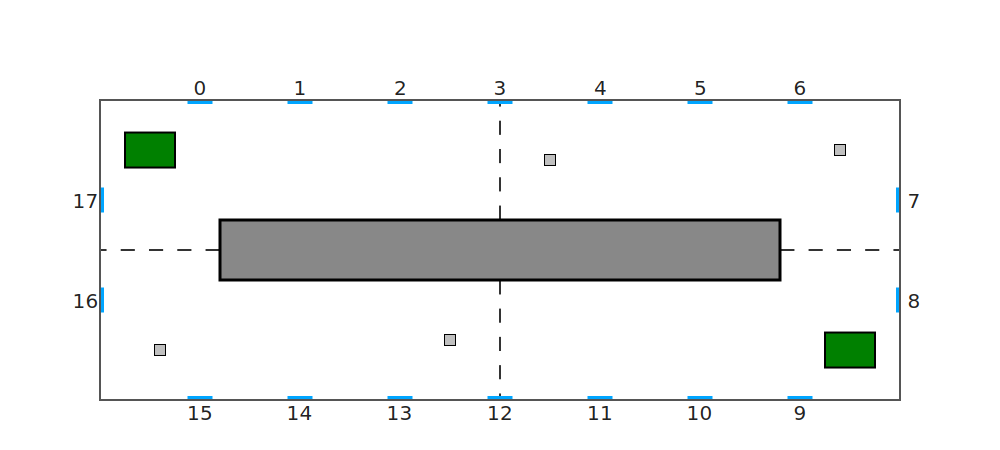
\includegraphics[scale=0.58]{fig-arena.pdf}
  \caption{Layout zones and tokens in the arena.}
  \label{fig:arena}
\end{figure}

\subsection{Tokens}
\refstepcounter{SpecID}
\label{spec:tokens}

\begin{enumerate}
  \item Tokens are cubic corrugated cardboard boxes, with sides of length
        \si{110}{mm} $\pm$ \si{10}{mm}.
  \item Each face of each token has a libkoki marker attached. The marker is
        identical on all six faces.
  \item The poison token will be styled to be visibly distinct from ordinary
        tokens. The manner of this styling is undefined: robots must rely on
        the libkoki markers to distinguish the poison token and ordinary
        tokens.
  \item The initial layout of tokens in the arena is given in
        Figure~\ref{fig:arena}.
\end{enumerate}

